\begin{figure}[h!]
\centering
 \subfloat[Baseline.]{
  \label{fig:baseline}
%  \includegraphics[width=.32\textwidth,clip,trim = 18mm 213mm 117mm 20mm]{figs/eps/sim-rread-lat.eps}}
   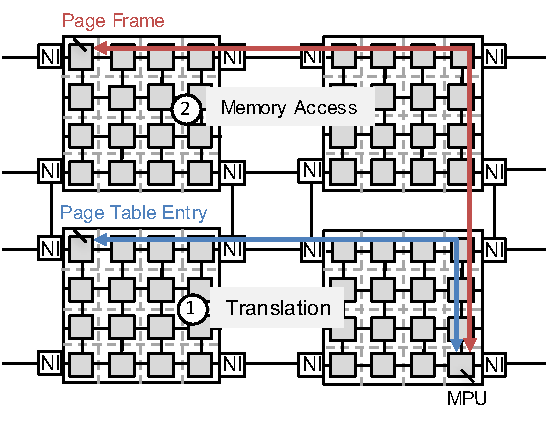
\includegraphics[clip,width=0.75\columnwidth]{figures/floorplan_vanilavm2.pdf}
%   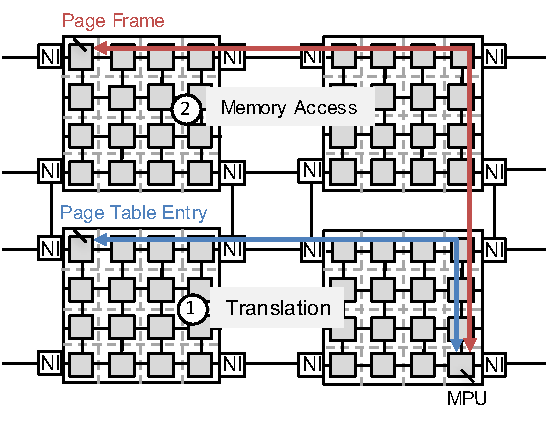
\includegraphics[width=0.69\columnwidth]{figures/floorplan_vanilavm2.pdf}}
   }
%  \hspace{.01in}

 \subfloat[Per-Chip MMU.]{
  \label{fig:chipmmu}
%  \includegraphics[width=.32\textwidth,clip,trim = 18mm 213mm 115mm 20mm]{figs/eps/sim-rread-bw.eps}}
 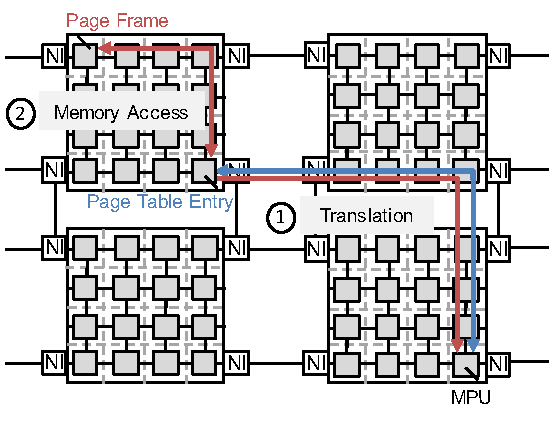
\includegraphics[clip,width=0.75\columnwidth]{figures/floorplan_chipvm2.pdf}
 %  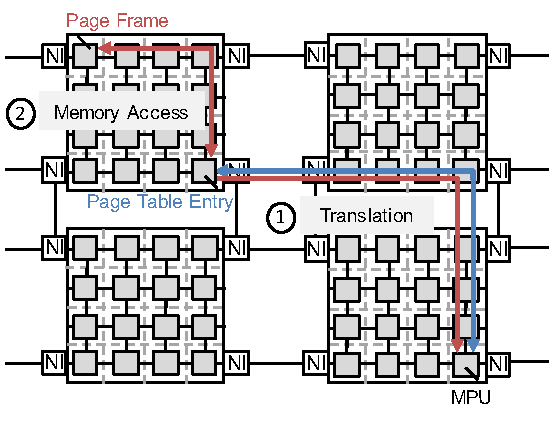
\includegraphics[width=0.69\columnwidth]{figures/floorplan_chipvm2.pdf}}
 }
% \hspace{.01in}

 \subfloat[Per-Partition MMU.]{
  \label{fig:partitionmmu}
%  \includegraphics[width=.32\textwidth,clip,trim = 18mm 213mm 115mm 20mm]{figs/eps/sim-rread-bw.eps}}
 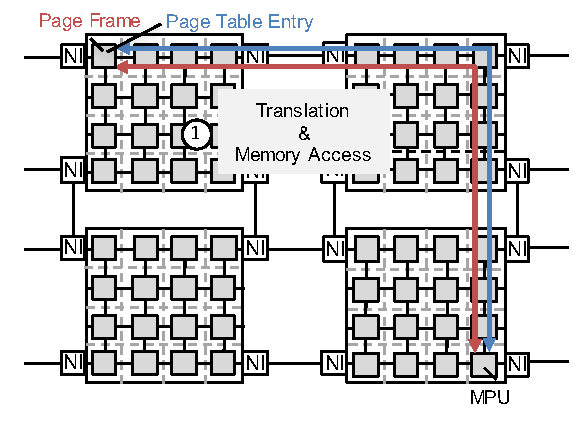
\includegraphics[clip,width=0.75\columnwidth]{figures/floorplan_partitionvm2.pdf}
%  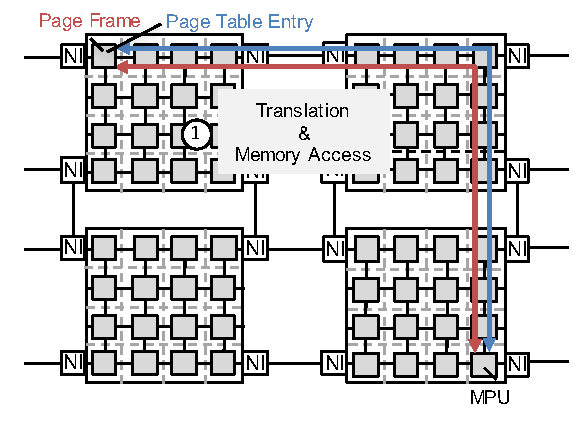
\includegraphics[width=0.695\columnwidth]{figures/floorplan_partitionvm2.pdf}}
 }

\caption{Different translation schemes on 4-chip floor plans. Large squares and small gray squares represent memory chips and partitions, respectively. Translation and memory access messages appear in blue and red, respectively. 
 \label{fig:translationSchemes_comparison}}
\end{figure}